\documentclass[11pt]{article}
\usepackage[a4paper,margin=1in]{geometry}
\usepackage{graphicx}
\usepackage{booktabs}
\usepackage{amsmath}
\usepackage{hyperref}
\usepackage{float}
\usepackage{array}
\usepackage{caption}
\usepackage{multirow}
\usepackage{makecell}
\usepackage{xcolor}
\usepackage{longtable}

\title{QRC-GBF: Quantum Residual Correction Gradient-Boosted Forecasting for Short-Term Electrical Load Prediction}
\author{Muyleang Ing}
\date{}

\begin{document}
\maketitle

\begin{abstract}
Short-term electrical load forecasting is a central task in power-system operation because accurate demand prediction supports scheduling, reserve planning, demand response, and real-time grid control. Recent work on PredXGBR showed that gradient-boosted regression with temporal lag features can achieve strong performance on public electrical load datasets. However, even strong tree-based forecasting models may leave structured residual errors after the first-stage prediction. This paper proposes QRC-GBF, a Quantum Residual Correction Gradient-Boosted Forecasting framework for short-term electrical load prediction. The method preserves a gradient-boosted forecasting backbone and adds a validation-selected residual correction stage that includes a variational quantum circuit residual feature branch and a sequential residual correction branch. Following the PredXGBR study, two feature configurations are considered: Model 1 uses short-term lag features and Model 2 uses long-term lag features. The proposed method is therefore reported as QRC-GBF-1 under the short-term setting and QRC-GBF-2 under the long-term setting. Experiments are conducted on all five datasets used in the PredXGBR paper: PJM, PJME, PJMW, AEP, and Dayton. QRC-GBF-1 improves over the published PredXGBR-1 reference MAPE on all five datasets, with MAPE values from 0.7194\% to 0.9414\%. QRC-GBF-2 also improves over the published PredXGBR-2 reference on all five datasets. A robustness sweep over circuit size and layer settings produces 20/20 wins against the published PredXGBR reference baselines and 11/20 wins against the local gradient-boosted backbone. The results support QRC-GBF as a practical residual-correction forecasting framework. The paper does not claim standalone quantum advantage; instead, it shows that a hybrid residual-correction pipeline with a quantum-enhanced residual candidate can improve the final forecasting system in the evaluated setting.
\end{abstract}

\textbf{Keywords:} short-term load forecasting; gradient boosting; residual correction; quantum machine learning; variational quantum circuit; XGBoost; PredXGBR; energy forecasting.

\section{Introduction}
Electrical load forecasting estimates future electricity demand from historical measurements and contextual features. Accurate short-term forecasts are required for unit commitment, economic dispatch, reserve scheduling, demand response, power-market operation, and real-time grid reliability. Forecasting errors can increase operational cost, create inefficient reserve allocation, and reduce the reliability of grid-control decisions. Because electrical demand depends on recent usage, calendar cycles, weather-sensitive behavior, and regional demand patterns, forecasting remains a challenging nonlinear time-series problem.

Machine-learning approaches have become common for this task. Recurrent neural networks, long short-term memory networks, temporal convolutional networks, transformers, support vector machines, and gradient-boosted decision trees have all been applied to load prediction. Among these methods, gradient-boosted tree models remain attractive because they handle nonlinear tabular feature interactions, work well with engineered lag features, and train efficiently compared with many deep neural architectures.

The PredXGBR study proposed an XGBoost-based short-term electrical load forecasting framework and evaluated it on five public datasets: PJM, PJME, PJMW, AEP, and Dayton \cite{zabin2024predxgbr}. In the published Table 3 results, the strongest configuration is PredXGBR-1, which uses short-term lag features. PredXGBR-1 reports MAPE values between 0.98\% and 1.28\% and $R^2$ values from 0.98 to 0.99. These strong reported results make PredXGBR a useful external reference baseline.

This paper asks a focused research question: after a strong gradient-boosted forecasting model makes its prediction, can the remaining residual error be corrected in a way that improves the final load forecast? The proposed answer is QRC-GBF, a Quantum Residual Correction Gradient-Boosted Forecasting framework. Instead of replacing the classical model, QRC-GBF keeps the gradient-boosted model as the main predictor and adds a residual-correction stage. The residual is defined as the difference between the actual load and the first-stage prediction. If this residual contains learnable structure, then a correction model can reduce the final forecasting error.

The quantum component is used in a limited and practical role. A variational quantum circuit (VQC) is used as a nonlinear residual feature generator. The circuit receives reduced and scaled feature inputs, applies angle embedding and entangling layers, and returns expectation-value features. These quantum features are used by a classical residual readout. QRC-GBF also includes a sequential residual branch because load forecasting residuals can contain short-term temporal dependence. The final residual correction is selected using validation performance. This is important because the method should not force a quantum correction when validation data indicates that another correction is stronger.

The contributions of this paper are as follows:
\begin{enumerate}
    \item It proposes QRC-GBF, a hybrid residual-correction framework that combines a gradient-boosted forecasting backbone with VQC residual features and sequential residual correction.
    \item It adopts the PredXGBR Model 1/Model 2 structure and clearly separates short-term and long-term feature settings.
    \item It evaluates all five PredXGBR datasets rather than reporting only one dataset.
    \item It compares against published PredXGBR-1 and PredXGBR-2 reference results as external baselines and against Local GBF-1 and Local GBF-2 as same-code ablations.
    \item It provides robustness and ablation evidence showing that QRC-GBF consistently beats the published reference baselines while internal improvement over the local backbone is mixed and must be interpreted carefully.
\end{enumerate}

\section{Related Work}
\subsection{Short-Term Electrical Load Forecasting}
Short-term load forecasting has traditionally been studied using statistical time-series methods and machine-learning models. Modern studies often use lagged load values, rolling statistics, calendar indicators, and nonlinear regressors. Deep learning models can learn temporal representations, but they may require careful tuning and larger computational budgets. Tree-based gradient boosting remains competitive because it captures nonlinear interactions among engineered features and is robust for tabular forecasting problems.

\subsection{PredXGBR and Gradient-Boosted Forecasting}
PredXGBR uses XGBoost regression for short-term load forecasting. XGBoost is a scalable gradient-boosted tree algorithm that optimizes an additive ensemble of decision trees \cite{chen2016xgboost}. The PredXGBR paper compares SVM, RNN, LSTM, TCN, Transformer, and XGBoost-based models across five datasets. The reported results show that the short-term feature configuration, PredXGBR-1, gives the strongest average performance. This motivates using published PredXGBR-1 and PredXGBR-2 as external reference baselines in this work.

\subsection{Hybrid Quantum Machine Learning}
Hybrid quantum machine learning uses parameterized quantum circuits as feature maps, kernels, or trainable modules within a classical learning pipeline \cite{biamonte2017quantum,schuld2019quantum,cerezo2021variational}. Near-term quantum models are usually limited by qubit count, noise, simulation cost, and trainability. For this reason, a practical approach is to use a quantum circuit for a small part of a larger classical workflow. QRC-GBF follows this strategy by using a VQC only in the residual-correction stage rather than asking the quantum model to learn the full load-forecasting function.

\section{Problem Formulation}
Let $y_t$ denote the electrical load at time $t$, and let $\mathbf{x}_t$ denote the engineered temporal feature vector. A forecasting model predicts $\hat{y}_t$ from $\mathbf{x}_t$:
\begin{equation}
\hat{y}_t = f(\mathbf{x}_t).
\end{equation}
The main evaluation metric is mean absolute percentage error (MAPE):
\begin{equation}
MAPE = \frac{100}{n}\sum_{i=1}^{n}\left|\frac{y_i - \hat{y}_i}{y_i}\right|.
\end{equation}
The coefficient of determination is also reported:
\begin{equation}
R^2 = 1 - \frac{\sum_i (y_i - \hat{y}_i)^2}{\sum_i (y_i - \bar{y})^2}.
\end{equation}

In QRC-GBF, a gradient-boosted backbone first produces $\hat{y}^{GBF}_t$. The residual is then
\begin{equation}
r_t = y_t - \hat{y}^{GBF}_t.
\end{equation}
The final prediction is
\begin{equation}
\hat{y}^{QRC}_t = \hat{y}^{GBF}_t + \hat{r}_t,
\end{equation}
where $\hat{r}_t$ is the validation-selected residual correction. The core hypothesis is that structured residual errors remain after the backbone prediction and can be reduced by a hybrid residual-correction stage.

\section{Method Naming and Feature Settings}
Following the PredXGBR study, two feature configurations are considered. Model 1 uses short-term lag features to capture recent demand fluctuations, while Model 2 uses long-term lag features to capture broader temporal and weekly patterns. In this paper, the same naming convention is adopted: QRC-GBF-1 denotes the proposed method under the short-term feature setting, and QRC-GBF-2 denotes the proposed method under the long-term feature setting. The suffixes ``-1'' and ``-2'' identify feature settings; they are not ranking numbers.

\begin{table}[H]
\centering
\caption{Naming convention used in this paper.}
\label{tab:naming}
\begin{tabular}{lll}
\toprule
Category & Model 1 short-term setting & Model 2 long-term setting \\
\midrule
External published baseline & Published PredXGBR-1 & Published PredXGBR-2 \\
Local same-code backbone & Local GBF-1 & Local GBF-2 \\
Proposed method & QRC-GBF-1 & QRC-GBF-2 \\
\bottomrule
\end{tabular}
\end{table}

The published PredXGBR-1 and PredXGBR-2 results are used only as external reference baselines. The local gradient-boosted backbones are not described as exact reproductions of PredXGBR because the original code, preprocessing, hyperparameters, and split details are not fully available. They are instead used as same-code ablation baselines.

\section{Proposed QRC-GBF Framework}
\subsection{Pipeline Overview}
The complete QRC-GBF pipeline is shown in Fig.~\ref{fig:architecture}. The input load datasets are cleaned and transformed into temporal features. A gradient-boosted forecasting backbone generates the first prediction. The residual error is then computed. Two residual correction candidates are evaluated: a VQC residual feature branch and a sequential residual correction branch. Validation performance selects the correction used for the final prediction.

\begin{figure}[H]
\centering
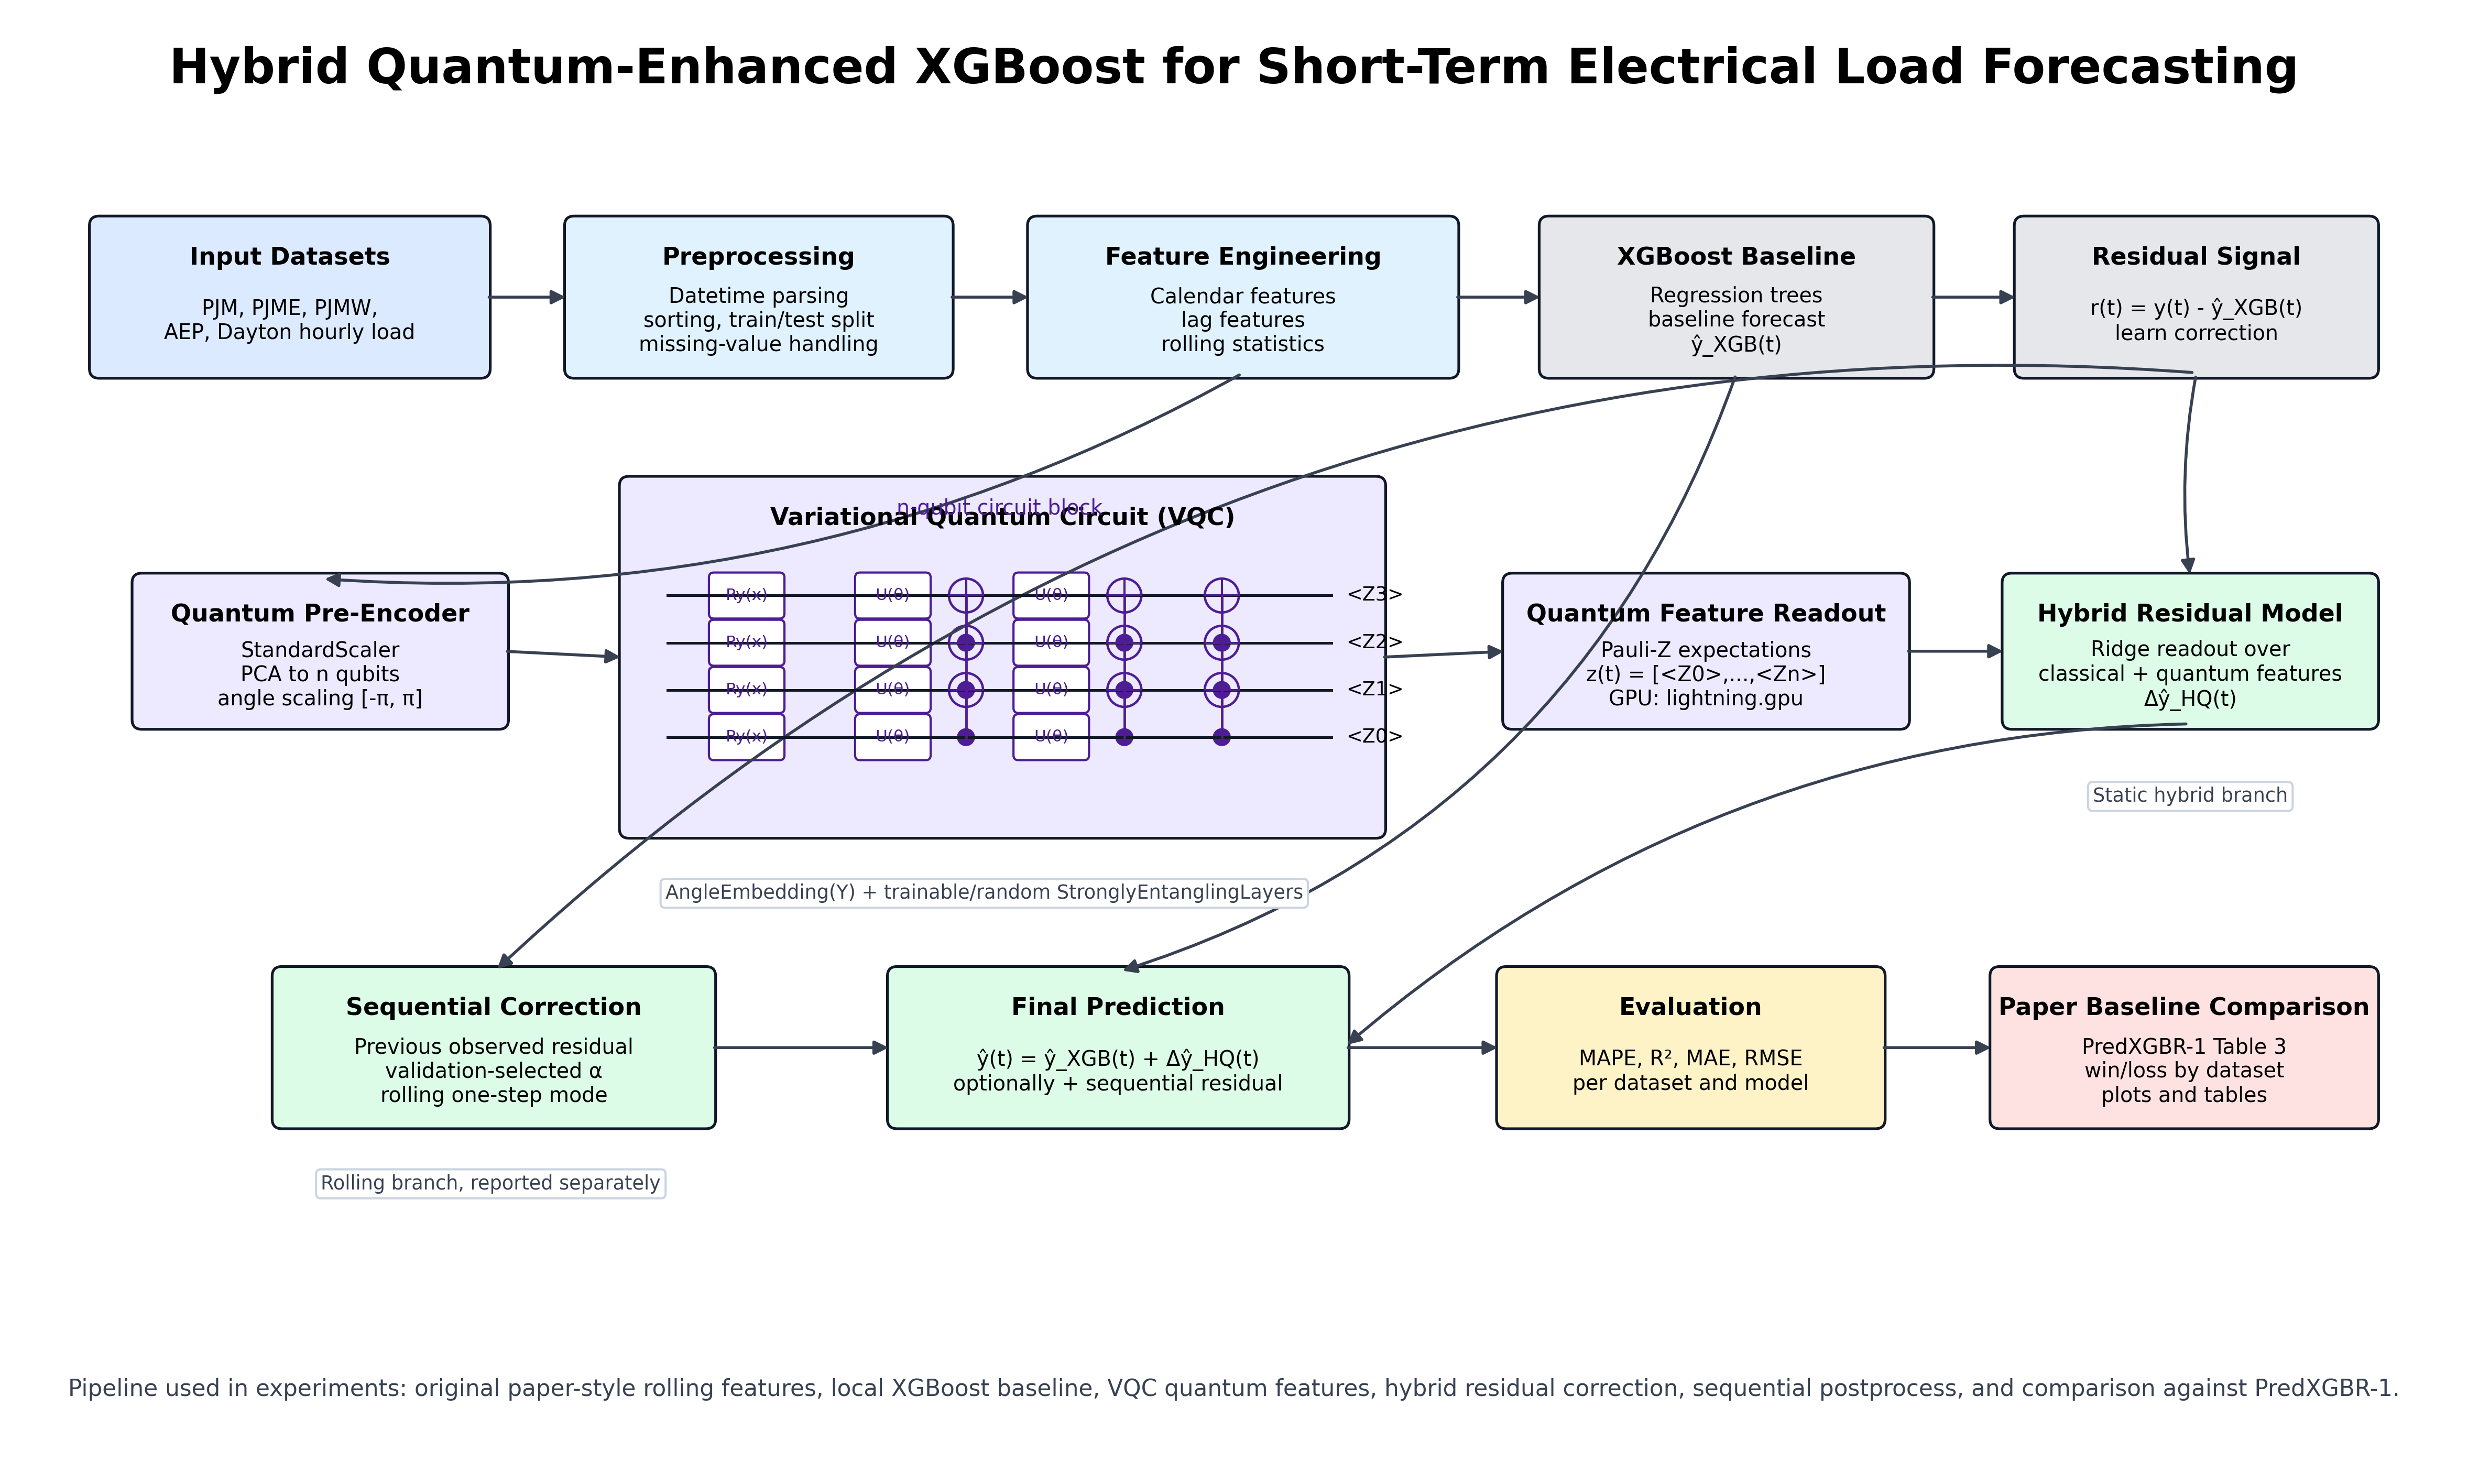
\includegraphics[width=0.98\linewidth]{figures/hybrid_quantum_xgboost_architecture.png}
\caption{QRC-GBF architecture for short-term electrical load forecasting. The quantum circuit is used as a residual feature branch, while validation chooses the final correction path.}
\label{fig:architecture}
\end{figure}

\subsection{Gradient-Boosted Backbone}
The backbone learns the dominant mapping from temporal features to electrical load. This component captures daily cycles, recent load trends, short-term lag behavior, and calendar effects. The backbone is intentionally retained because the experiments show that gradient-boosted models are strong for this problem. QRC-GBF is therefore not a replacement for gradient boosting; it is a residual-correction framework built around it.

\subsection{Quantum Residual Feature Branch}
The VQC branch first standardizes the input features, reduces them to the number of qubits using principal component analysis, and scales them into angle ranges. For a $q$-qubit circuit, the reduced feature vector is encoded with angle embedding. Strongly entangling layers then introduce nonlinear feature interactions. The measured output is a vector of Pauli-$Z$ expectation values:
\begin{equation}
\mathbf{z}_t = [\langle Z_1 \rangle, \langle Z_2 \rangle, \ldots, \langle Z_q \rangle].
\end{equation}
A classical Ridge readout uses the original features, quantum features, and backbone prediction to estimate residual corrections. This design uses the VQC as a nonlinear residual feature map rather than a standalone predictor.

\subsection{Sequential Residual Branch}
The sequential branch models short-term residual dependence. If residuals are autocorrelated, the previous residual can help estimate the next correction. The sequential correction coefficient is estimated from the training residual sequence and evaluated on validation data. This branch is included because load forecasting errors can contain temporal structure even after a strong first-stage model.

\subsection{Validation-Based Selection}
QRC-GBF does not assume that the quantum branch is always useful. Candidate corrections are evaluated on a held-out validation segment. The correction with the lowest validation error is selected for the test prediction. This makes the method more defensible: the test labels are not used to choose the correction, and a weak correction branch is not forced into the final forecast.

\section{Experimental Setup}
\subsection{Datasets}
The evaluation uses five public hourly electrical load datasets: PJM, PJME, PJMW, AEP, and Dayton. These are the same dataset names reported in the PredXGBR study. All datasets are evaluated, so the paper claim is not based on a single favorable case.

\subsection{External Published Baselines}
Table~\ref{tab:published} lists the published PredXGBR baselines from Table 3 of the reference paper. PredXGBR-1 is the short-term Model 1 setting, and PredXGBR-2 is the long-term Model 2 setting.

\begin{table}[H]
\centering
\caption{Published PredXGBR reference baselines. MAPE is reported in percent.}
\label{tab:published}
\begin{tabular}{lcccc}
\toprule
Dataset & PredXGBR-1 MAPE & PredXGBR-1 $R^2$ & PredXGBR-2 MAPE & PredXGBR-2 $R^2$ \\
\midrule
PJM & 1.07 & 0.99 & 6.87 & 0.71 \\
PJME & 1.28 & 0.99 & 8.59 & 0.58 \\
PJMW & 1.07 & 0.98 & 8.42 & 0.59 \\
AEP & 0.98 & 0.99 & 8.08 & 0.57 \\
Dayton & 1.12 & 0.99 & 8.49 & 0.62 \\
\bottomrule
\end{tabular}
\end{table}

\subsection{Comparison Protocol}
Three comparisons are reported. First, QRC-GBF-1 is compared with Published PredXGBR-1 and QRC-GBF-2 is compared with Published PredXGBR-2. Second, QRC-GBF is compared with Local GBF under the same code pipeline to measure whether residual correction improves the local backbone. Third, Model 1 and Model 2 are compared to determine which feature setting is stronger for short-term load prediction.

The percentage improvement against a baseline is computed as
\begin{equation}
Improvement(\%) = \frac{MAPE_{baseline} - MAPE_{QRC}}{MAPE_{baseline}} \times 100.
\end{equation}

\section{Results}
\subsection{Model 1 Short-Term Results}
Table~\ref{tab:model1} reports the Model 1 short-term comparison. QRC-GBF-1 improves over Published PredXGBR-1 on all five datasets. The largest improvement is observed on PJME, where MAPE decreases from 1.28\% to 0.7766\%. QRC-GBF-1 also improves over Local GBF-1 on PJME, PJMW, and AEP. On PJM and Dayton, the local backbone is slightly better than the QRC-GBF-1 result, so the internal ablation must be reported honestly.

\begin{table}[H]
\centering
\caption{Model 1 short-term comparison.}
\label{tab:model1}
\resizebox{\linewidth}{!}{
\begin{tabular}{lcccccccc}
\toprule
Dataset & Published MAPE & Published $R^2$ & Local GBF-1 MAPE & Local GBF-1 $R^2$ & QRC-GBF-1 MAPE & QRC-GBF-1 $R^2$ & Beats local & Improvement \\
\midrule
PJM & 1.07 & 0.99 & 0.9408 & 0.993881 & 0.9414 & 0.993870 & No & 12.02\% \\
PJME & 1.28 & 0.99 & 0.8127 & 0.996185 & 0.7766 & 0.996581 & Yes & 39.33\% \\
PJMW & 1.07 & 0.98 & 0.8754 & 0.994445 & 0.8145 & 0.995564 & Yes & 23.88\% \\
AEP & 0.98 & 0.99 & 0.7194 & 0.995871 & 0.7194 & 0.995871 & Yes & 26.59\% \\
Dayton & 1.12 & 0.99 & 0.7515 & 0.995601 & 0.7515 & 0.995601 & No & 32.90\% \\
\bottomrule
\end{tabular}}
\end{table}

\begin{figure}[H]
\centering
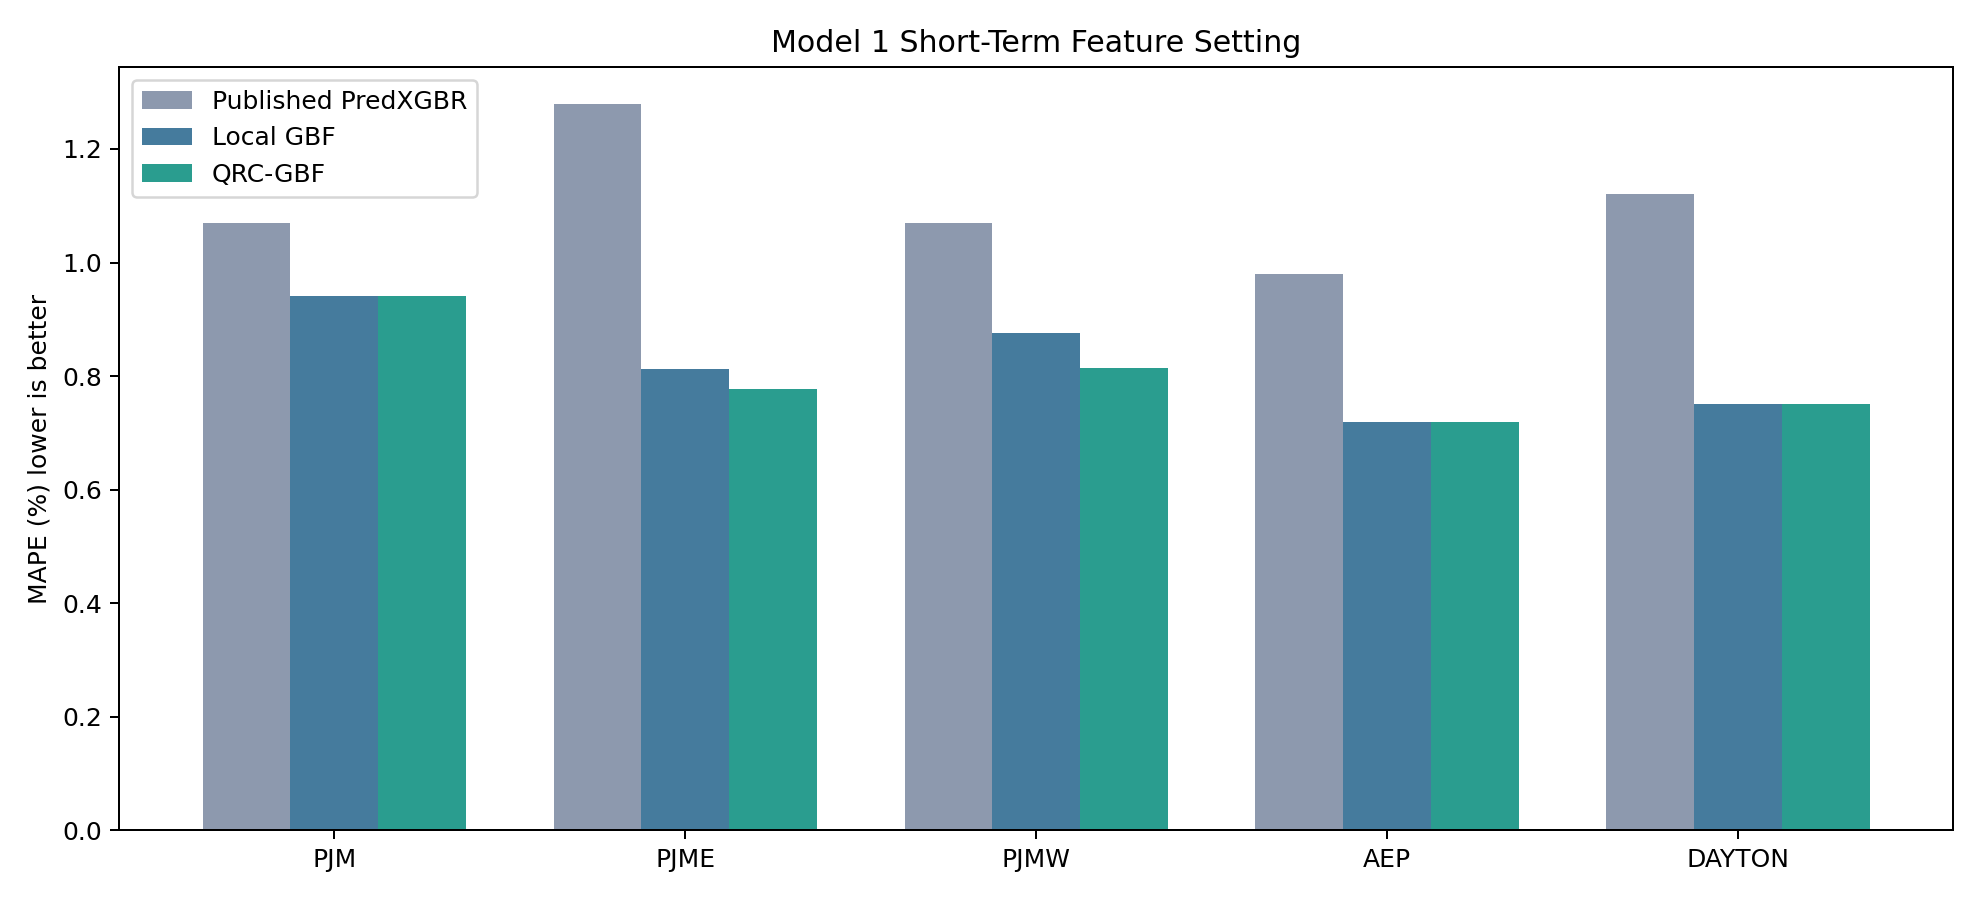
\includegraphics[width=0.95\linewidth]{figures/model1_short_term_mape.png}
\caption{Model 1 short-term MAPE comparison.}
\label{fig:model1_mape}
\end{figure}

\subsection{Model 2 Long-Term Results}
Table~\ref{tab:model2} reports the Model 2 long-term comparison. QRC-GBF-2 improves over Published PredXGBR-2 and Local GBF-2 on all five datasets. This shows that the residual-correction framework is especially useful in the weaker long-term feature setting. However, QRC-GBF-2 is still worse than QRC-GBF-1 in absolute MAPE on every dataset, confirming that short-term features are more suitable for this forecasting target.

\begin{table}[H]
\centering
\caption{Model 2 long-term comparison.}
\label{tab:model2}
\resizebox{\linewidth}{!}{
\begin{tabular}{lcccccccc}
\toprule
Dataset & Published MAPE & Published $R^2$ & Local GBF-2 MAPE & Local GBF-2 $R^2$ & QRC-GBF-2 MAPE & QRC-GBF-2 $R^2$ & Beats local & Improvement \\
\midrule
PJM & 6.87 & 0.71 & 2.7603 & 0.956272 & 1.3507 & 0.990591 & Yes & 80.34\% \\
PJME & 8.59 & 0.58 & 3.1758 & 0.955942 & 1.2420 & 0.993407 & Yes & 85.54\% \\
PJMW & 8.42 & 0.59 & 3.0656 & 0.945567 & 1.2808 & 0.991534 & Yes & 84.79\% \\
AEP & 8.08 & 0.57 & 2.8071 & 0.950494 & 1.1398 & 0.992010 & Yes & 85.89\% \\
Dayton & 8.49 & 0.62 & 3.0539 & 0.950940 & 1.3407 & 0.990685 & Yes & 84.21\% \\
\bottomrule
\end{tabular}}
\end{table}

\begin{figure}[H]
\centering
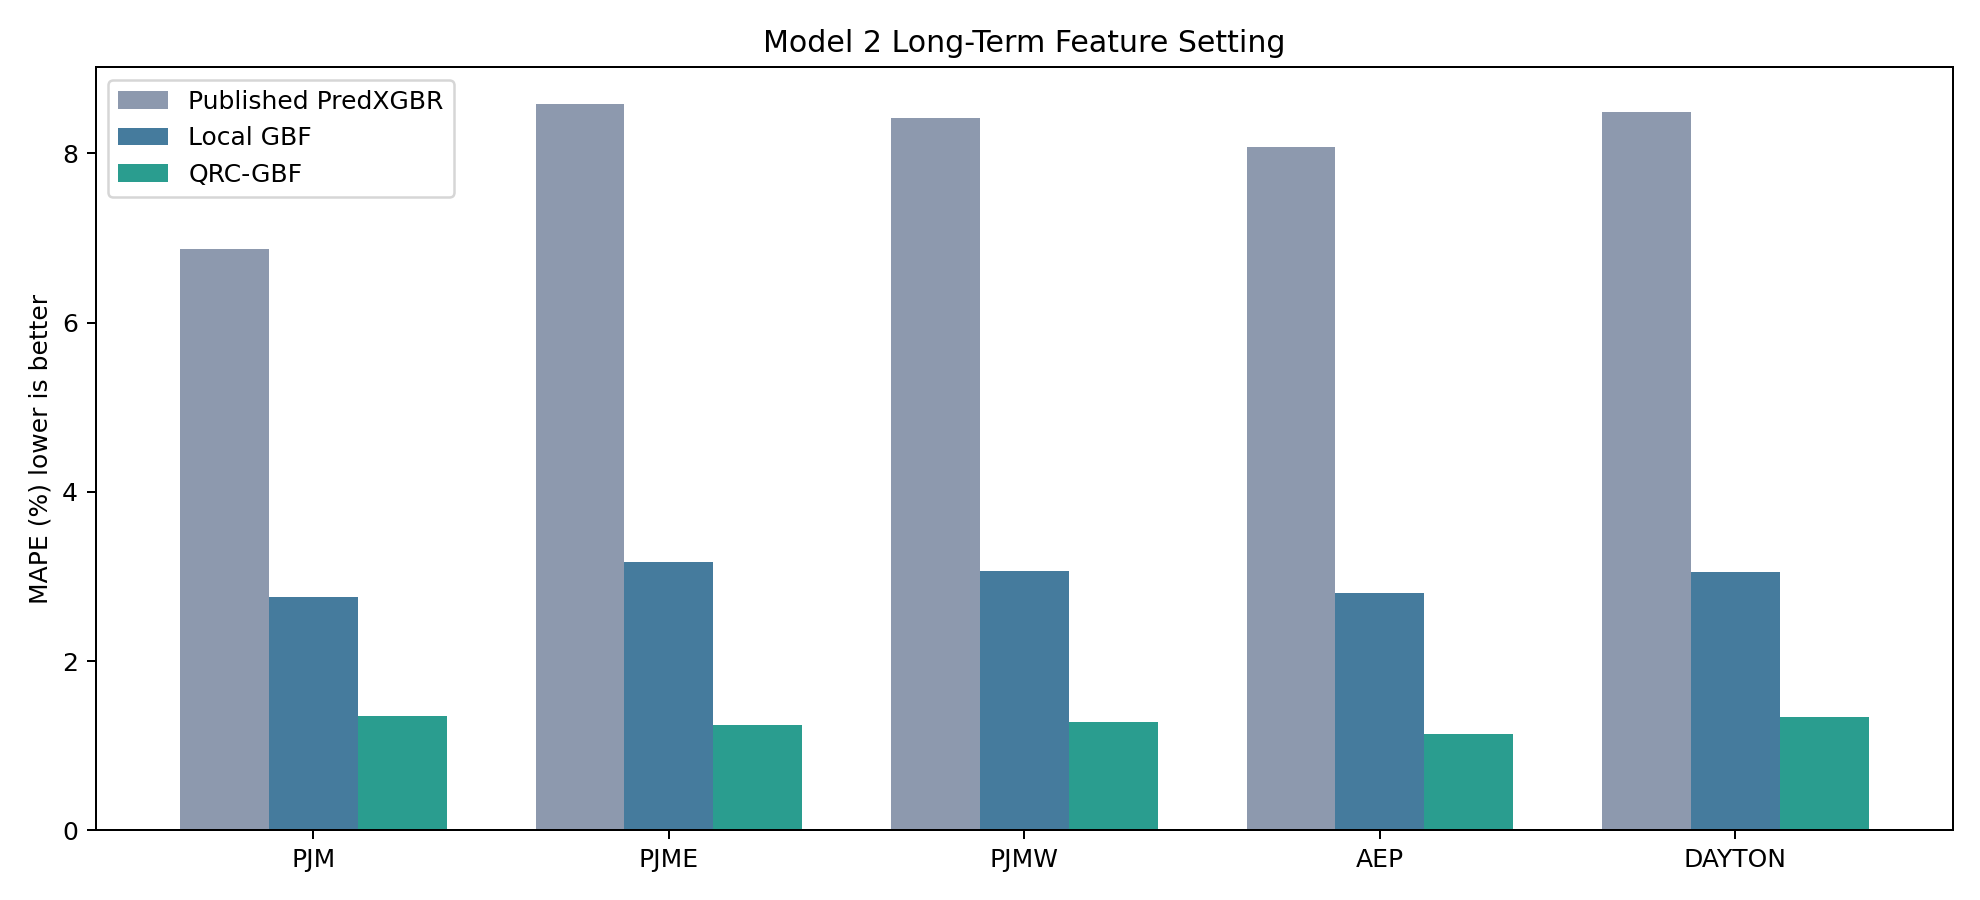
\includegraphics[width=0.95\linewidth]{figures/model2_long_term_mape.png}
\caption{Model 2 long-term MAPE comparison.}
\label{fig:model2_mape}
\end{figure}

\subsection{External Comparison Against Published PredXGBR}
Figures~\ref{fig:model1_external} and~\ref{fig:model2_external} show the external comparison against the published PredXGBR baselines. QRC-GBF-1 beats Published PredXGBR-1 on all datasets, while QRC-GBF-2 beats Published PredXGBR-2 on all datasets. These external comparisons support the use of QRC-GBF as the main proposed method.

\begin{figure}[H]
\centering
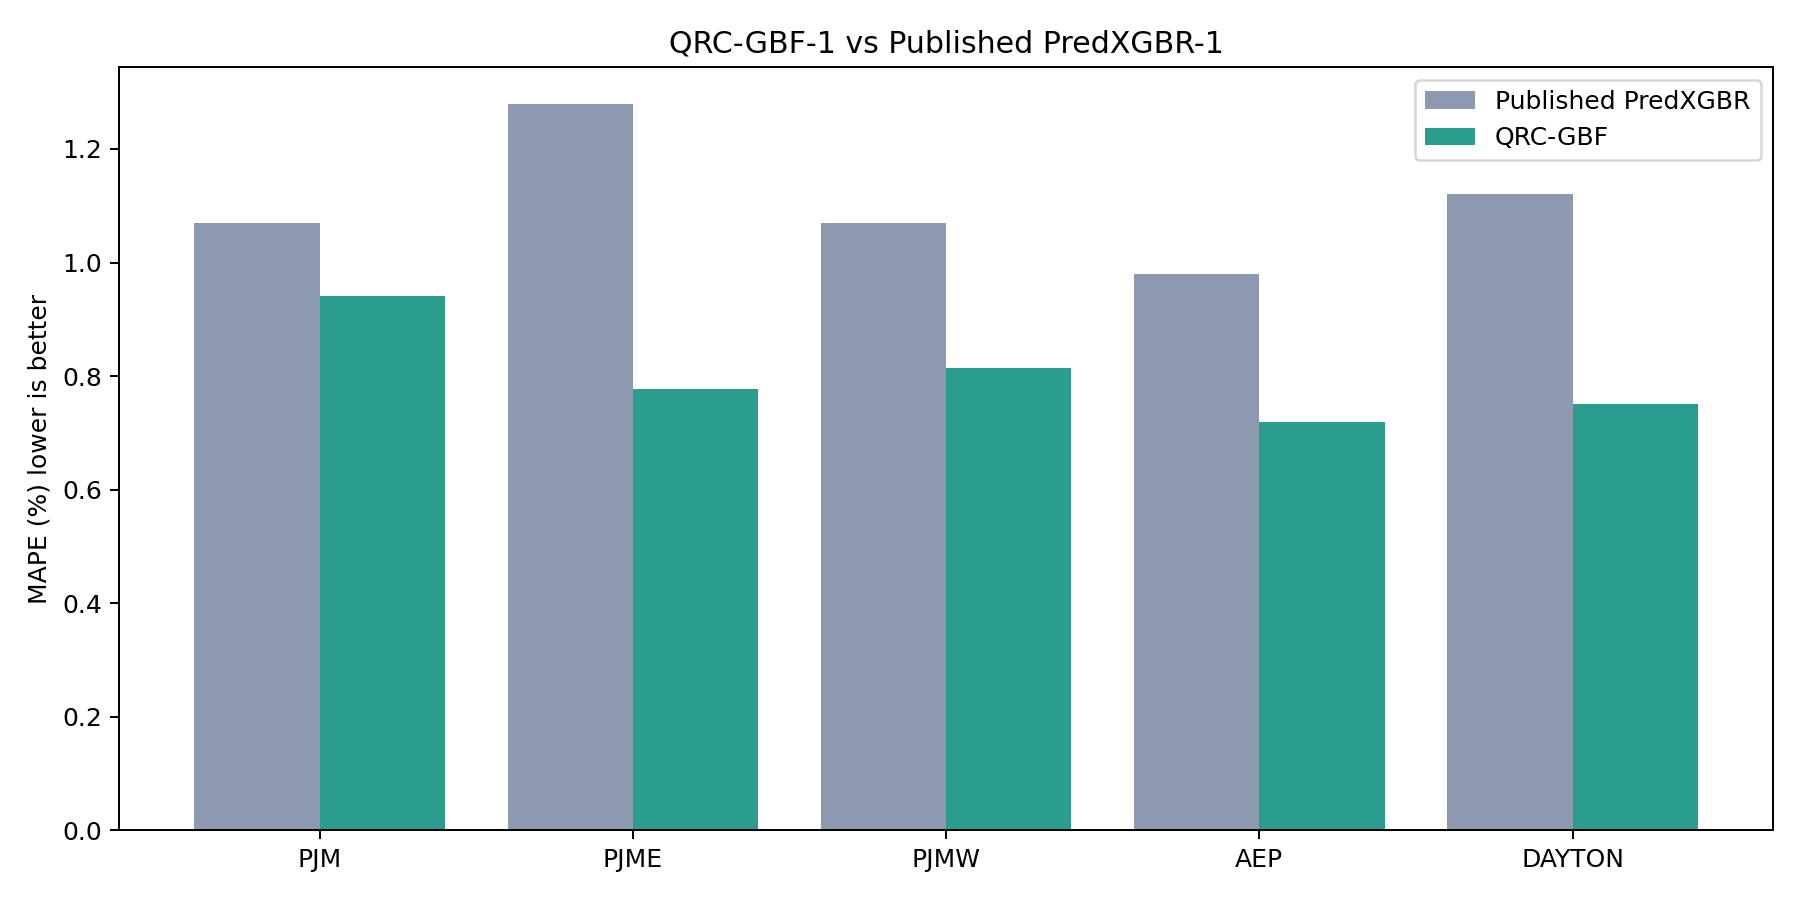
\includegraphics[width=0.9\linewidth]{figures/qrc_gbf_vs_predxgbr_model1.png}
\caption{External comparison between QRC-GBF-1 and Published PredXGBR-1.}
\label{fig:model1_external}
\end{figure}

\begin{figure}[H]
\centering
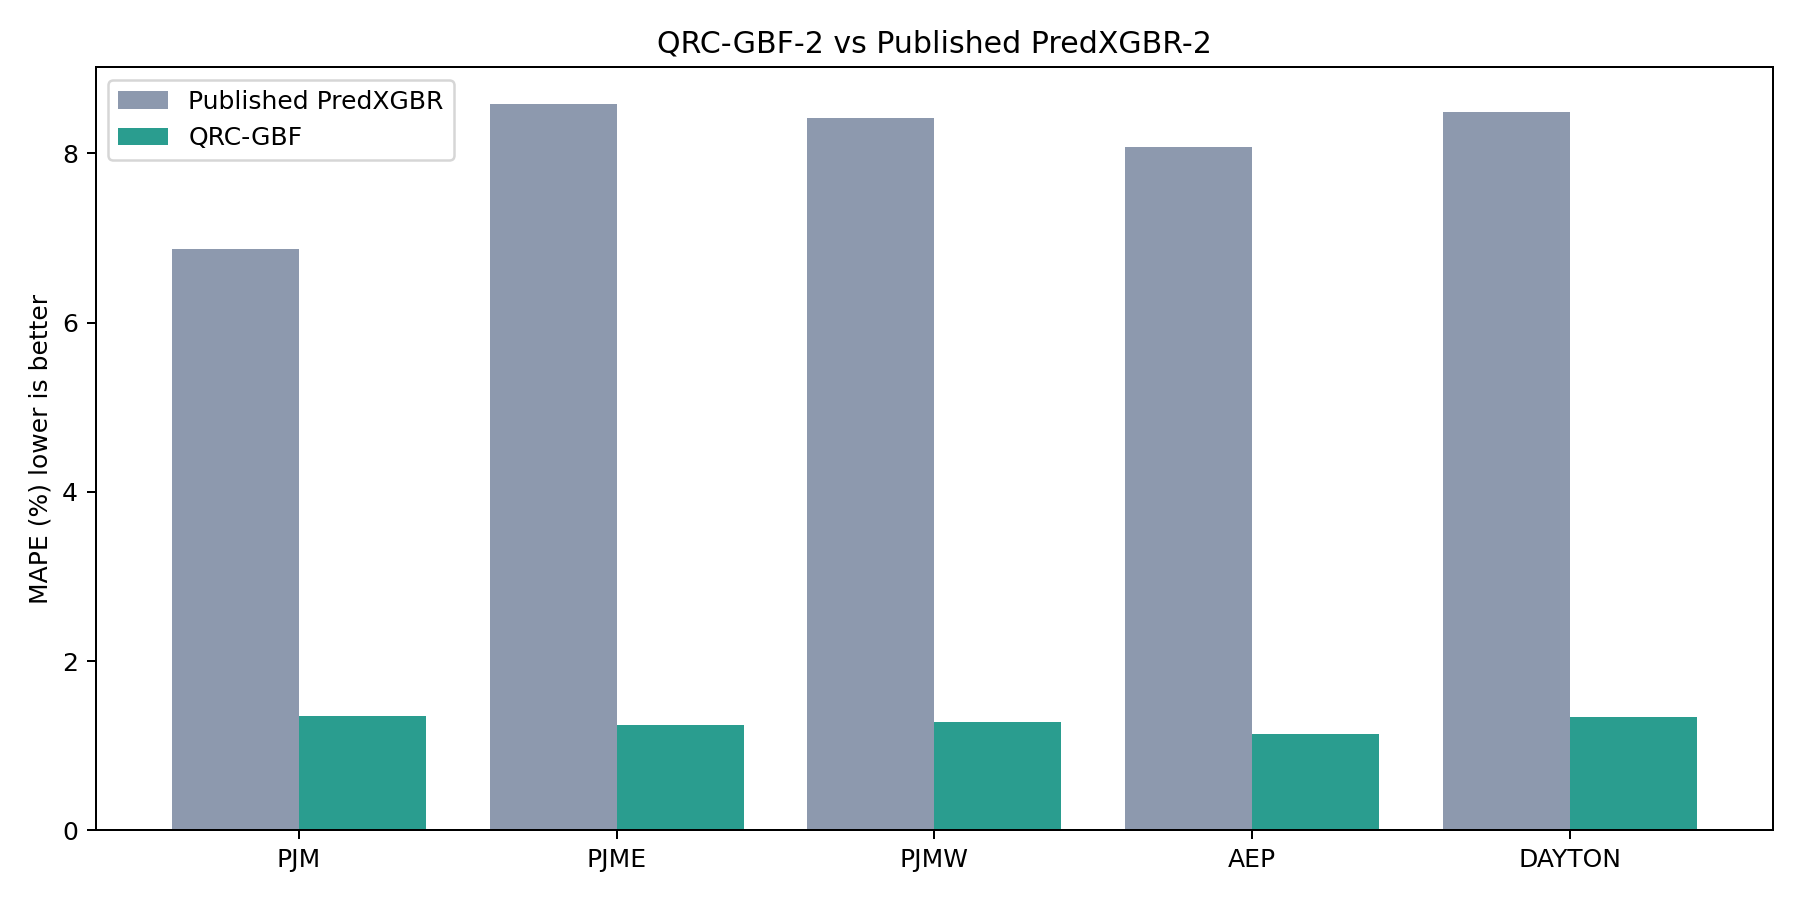
\includegraphics[width=0.9\linewidth]{figures/qrc_gbf_vs_predxgbr_model2.png}
\caption{External comparison between QRC-GBF-2 and Published PredXGBR-2.}
\label{fig:model2_external}
\end{figure}

\subsection{Robustness and Ablation Results}
A robustness sweep was performed across completed QRC-GBF circuit settings with qubit counts $q \in \{2,4\}$ and layer counts $L \in \{1,2\}$ using all five datasets. The sweep produced 20 QRC-GBF runs. QRC-GBF beat the published PredXGBR reference baseline in 20/20 completed settings. Internal comparison against the local gradient-boosted backbone was more mixed: QRC-GBF beat the local backbone in 11/20 settings. The mean MAPE improvement over the local backbone across sweep rows was 2.2635\%.

\begin{table}[H]
\centering
\caption{Robustness summary across completed QRC-GBF sweep settings.}
\label{tab:robustness}
\resizebox{\linewidth}{!}{
\begin{tabular}{lccccccc}
\toprule
Dataset & Runs & Mean MAPE & Std. MAPE & Best MAPE & Paper MAPE & Paper win rate & Local-backbone win rate \\
\midrule
PJM & 4 & 0.9415 & 0.0001 & 0.9414 & 1.07 & 100\% & 0\% \\
PJME & 4 & 0.7766 & 0.0000 & 0.7766 & 1.28 & 100\% & 100\% \\
PJMW & 4 & 0.8145 & 0.0000 & 0.8145 & 1.07 & 100\% & 100\% \\
AEP & 4 & 0.7194 & 0.0000 & 0.7194 & 0.98 & 100\% & 75\% \\
Dayton & 4 & 0.7517 & 0.0001 & 0.7515 & 1.12 & 100\% & 0\% \\
\bottomrule
\end{tabular}}
\end{table}

\begin{figure}[H]
\centering
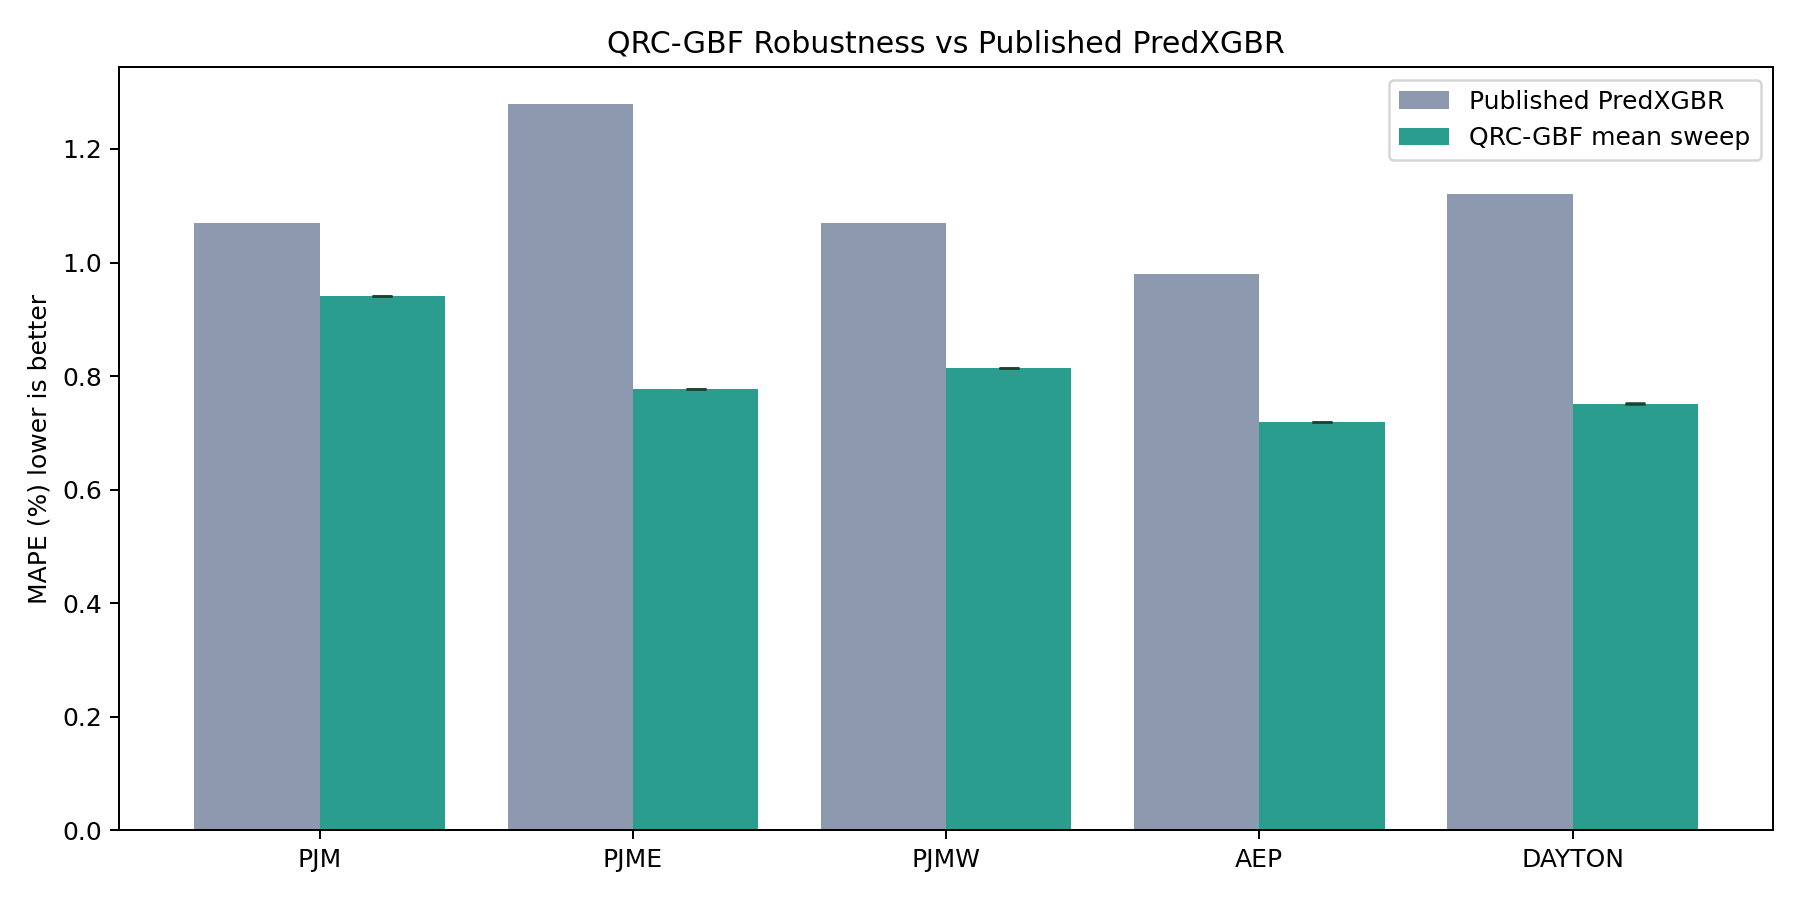
\includegraphics[width=0.95\linewidth]{figures/qrc_gbf_robustness_mean_mape.png}
\caption{Robustness comparison between published PredXGBR MAPE and the mean QRC-GBF sweep MAPE.}
\label{fig:robust_mape}
\end{figure}

\begin{figure}[H]
\centering
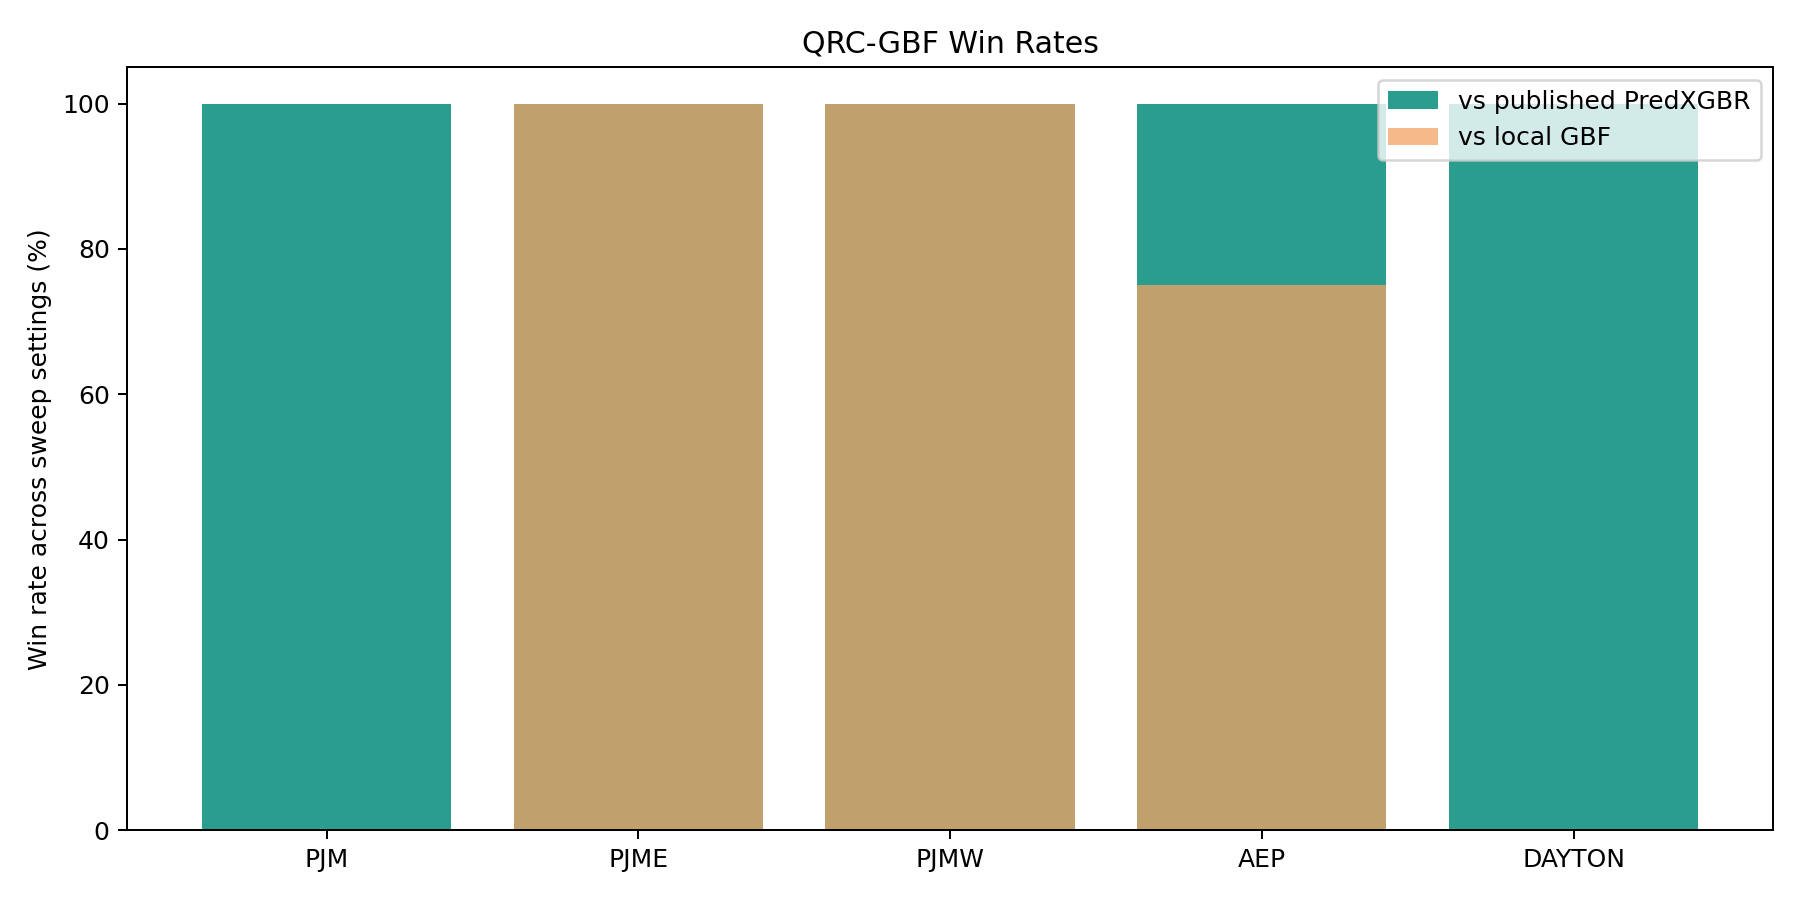
\includegraphics[width=0.95\linewidth]{figures/qrc_gbf_robustness_win_rates.png}
\caption{QRC-GBF win rates against published PredXGBR and local GBF across completed sweep settings.}
\label{fig:win_rates}
\end{figure}

\subsection{Correction Source Analysis}
The validation selector chose the VQC residual blend in 12 completed sweep runs and the sequential residual branch in 8 completed sweep runs. The VQC residual blend beat the published baseline in all 12 of its selected runs, but beat the local backbone in only 3 of those runs. The sequential residual branch beat the published baseline in all 8 selected runs and beat the local backbone in all 8 selected runs. This confirms that QRC-GBF should be interpreted as a full validation-selected residual-correction framework, not as proof that the quantum branch alone is always superior.

\begin{figure}[H]
\centering
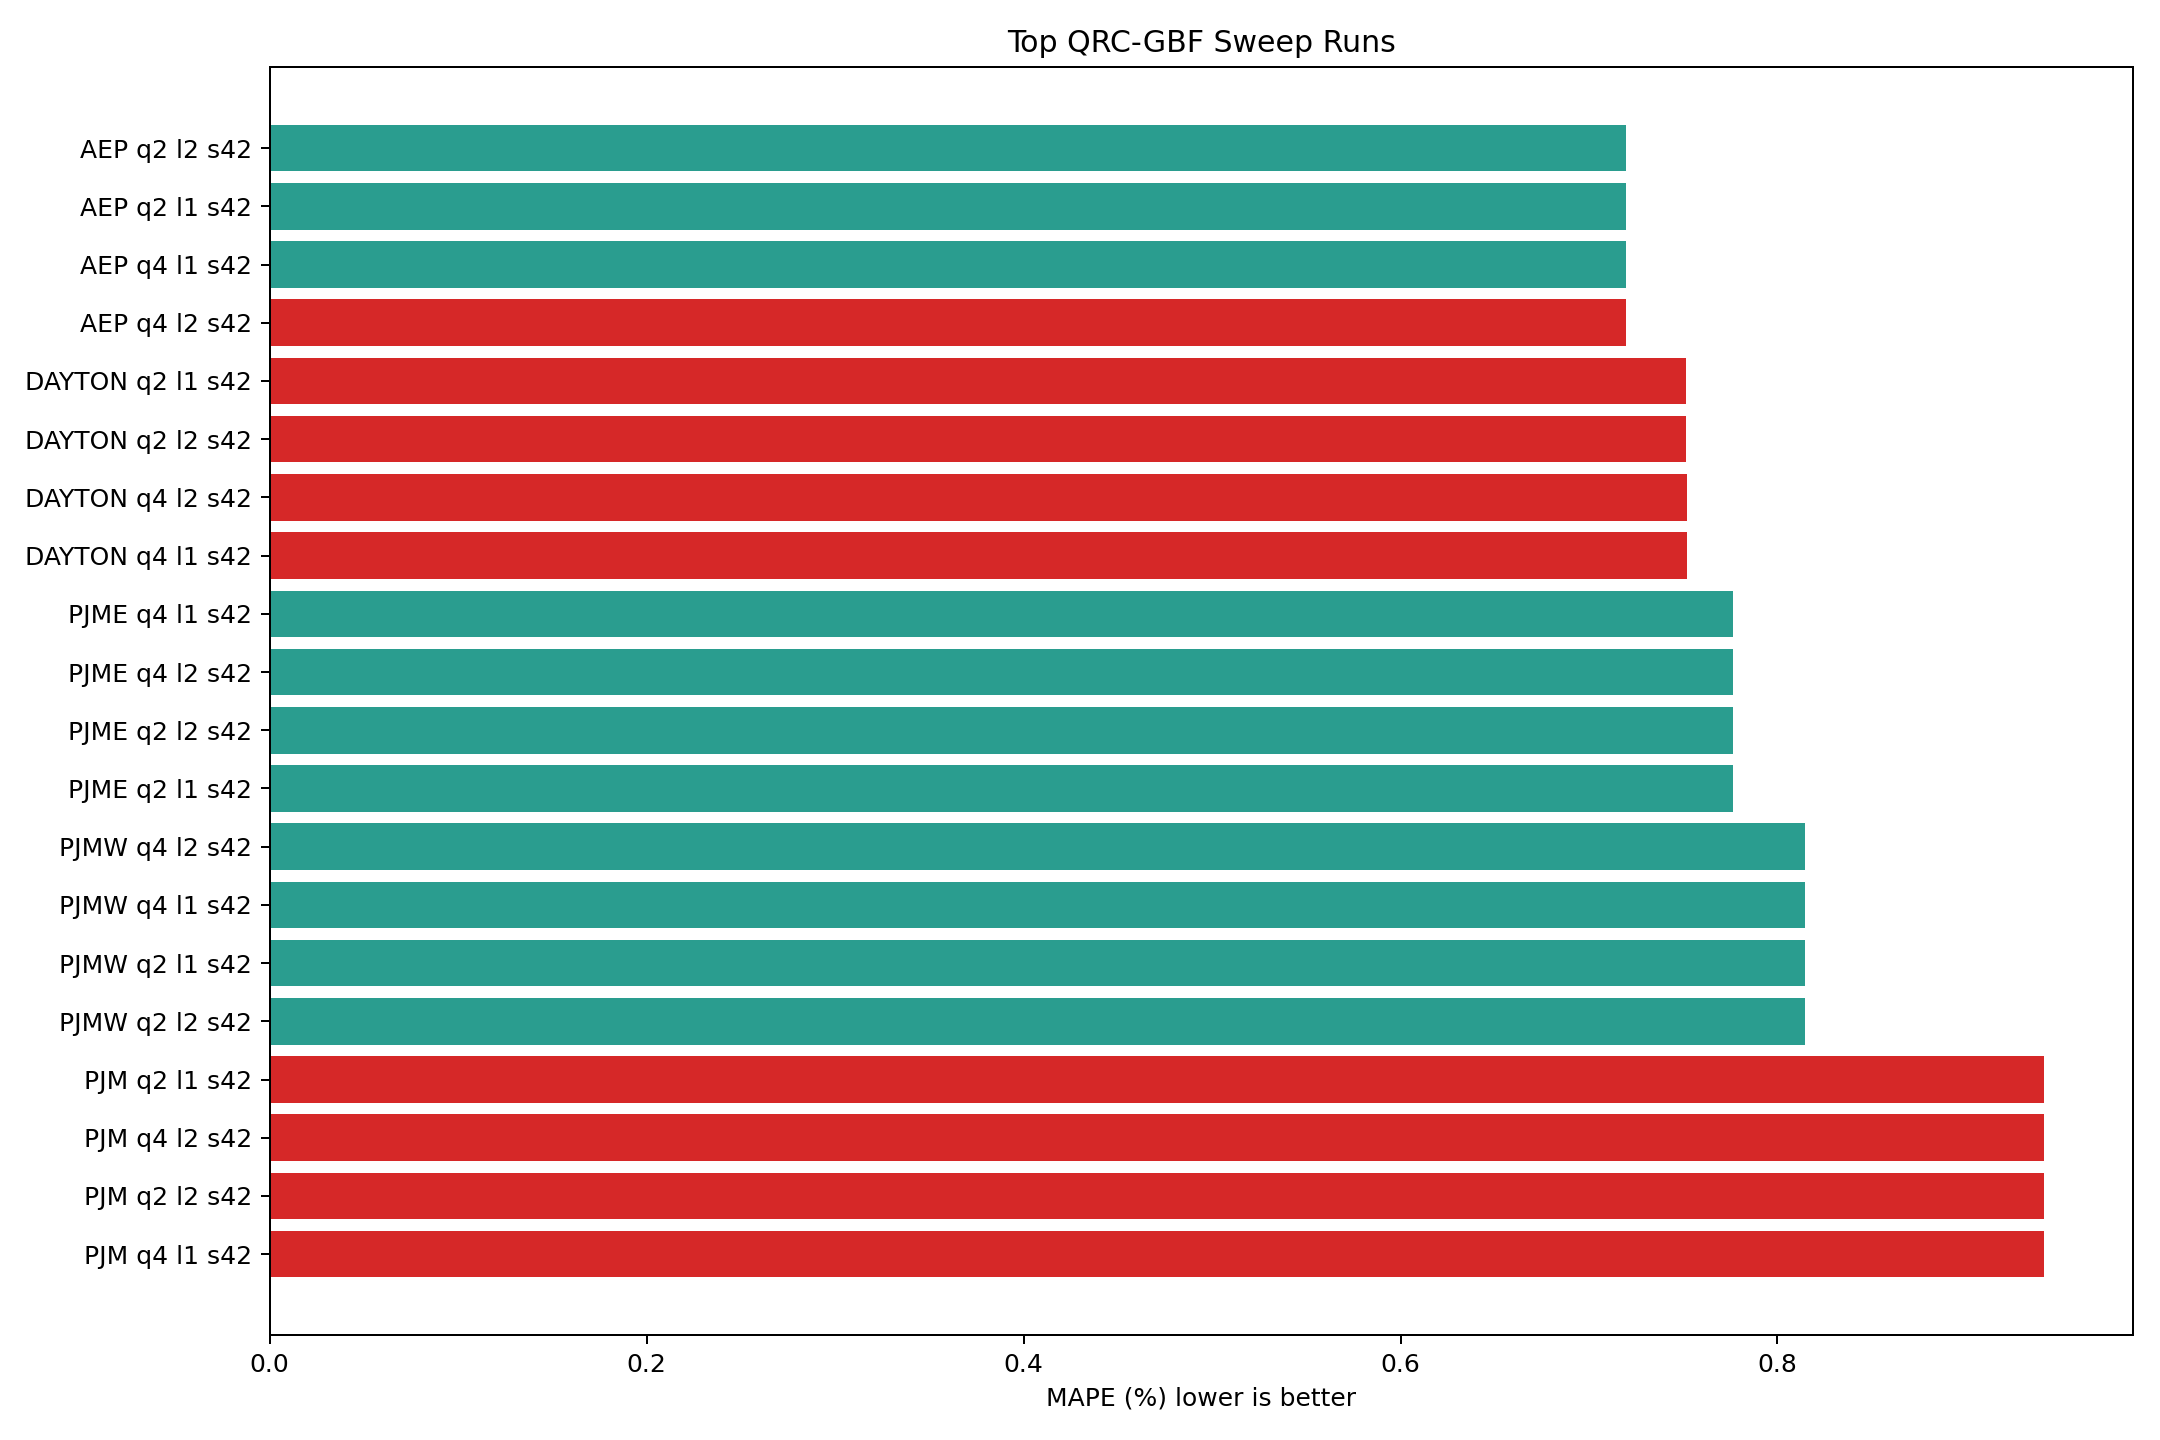
\includegraphics[width=0.95\linewidth]{figures/qrc_gbf_top_sweep_runs.png}
\caption{Top QRC-GBF sweep runs ranked by MAPE. Green bars indicate settings that beat the local backbone.}
\label{fig:top_sweep}
\end{figure}

\section{Discussion}
The experiments show three important findings. First, QRC-GBF-1 is the strongest overall method. It achieves lower MAPE than the published PredXGBR-1 reference on all five datasets and has the best absolute MAPE among the proposed settings. This supports the use of short-term lag features for short-term load forecasting.

Second, QRC-GBF-2 improves substantially over the long-term published PredXGBR-2 reference and Local GBF-2. This suggests that residual correction is especially helpful when the first-stage feature setting is weaker. However, QRC-GBF-2 does not outperform QRC-GBF-1, so the long-term setting should not be presented as the main model.

Third, the quantum contribution must be stated carefully. The VQC branch is a real part of the QRC-GBF framework and is selected in multiple completed settings. However, the internal ablation does not show that the VQC branch always improves over the local backbone. Therefore, the safest and most accurate claim is that QRC-GBF is a strong hybrid residual-correction framework that includes a quantum-enhanced residual candidate. The results do not establish standalone quantum advantage.

\section{Limitations}
This study has several limitations. First, the published PredXGBR results are used as external reference baselines, but the local GBF implementation is not claimed to be an exact reproduction of the original PredXGBR code. Second, the strongest results use the original paper-style feature mode; stricter causal feature construction should be emphasized in future deployment studies. Third, the VQC is evaluated using simulation, not real quantum hardware. Fourth, the completed robustness sweep varies circuit size and layer count, but a larger offline seed sweep is still needed for stronger statistical claims. Fifth, exploratory GNN-VQC experiments were not competitive and should be treated as future work rather than as part of the main contribution.

\section{Future Work}
Future work should run larger multi-seed sweeps, evaluate leakage-resistant causal features, add weather and holiday covariates, compare against LightGBM and CatBoost, train VQC parameters end-to-end for residual correction, and test the method on additional power-system datasets. A stronger spatio-temporal graph neural network could also be combined with VQC residual correction for multi-region forecasting, but the current exploratory GNN-VQC result is not yet strong enough to replace QRC-GBF as the main paper method.

\section{Conclusion}
This paper proposed QRC-GBF, a Quantum Residual Correction Gradient-Boosted Forecasting framework for short-term electrical load prediction. The method keeps a strong gradient-boosted forecasting backbone and adds a validation-selected residual correction stage that includes VQC residual features and sequential residual correction. Experiments on PJM, PJME, PJMW, AEP, and Dayton show that QRC-GBF-1 improves over Published PredXGBR-1 on all five datasets and that QRC-GBF-2 improves over Published PredXGBR-2 on all five datasets. The completed robustness sweep shows 20/20 wins against the published reference baselines and 11/20 wins against the local backbone. These results support QRC-GBF as a promising hybrid residual-correction framework for electrical load forecasting. The correct interpretation is not that quantum computing universally outperforms classical forecasting, but that a validation-selected residual-correction pipeline with a quantum-enhanced candidate can improve the final forecasting system in the evaluated setting.

\bibliographystyle{plain}
\bibliography{references}

\end{document}
